\documentclass[fontset=windows]{article}
\PassOptionsToPackage{quiet}{fontspec}
\usepackage[a4paper, total={6.5in, 10in}]{geometry}
\usepackage[format=hang,font=small,textfont=it]{caption}
\usepackage{lmodern}
\usepackage{mathtools}
\usepackage{amsmath}
\usepackage{array}
\usepackage{ctex}
\usepackage[toc,lof]{multitoc}  % 设置目录为多列
\usepackage{cancel}
% \usepackage{xeCJK}
%     \xeCJKsetup{CJKMath=true}
\usepackage{float}
\usepackage{pifont}
\usepackage{graphicx}
\usepackage{tcolorbox}
% \usepackage{tikz}
\usepackage{tikzit}
\usepackage{xcolor}
\usepackage[nottoc]{tocbibind}
\usepackage[hidelinks]{hyperref}
\usepackage{listings}
\newtheorem{theorem}{Theorem}
\newtheorem{lemma}{Lemma}
\newtheorem{proof}{Proof}[section]
\newtheorem{thm}{定理}
\newcommand\degree{^\circ}
\definecolor{lightblue}{HTML}{6495ED}
% \renewcommand{\textcircled}[1]{\ensuremath{\textcircled{#1}}}
\newcommand*{\mycircled}[1]{\lower
.7ex\hbox{\tikz\draw (0pt, 0pt) circle
(.4em) node {\makebox[0.5em][c]
{\small #1}};}}

\newenvironment{questions}
    {\begin{quote}
		\songti
		\zihao{-5}
	}
	{\end{quote}}

\newenvironment{QuoteEnv}[2][]
    {\newcommand\Qauthor{#1}\newcommand\Qref{#2}\zihao{-5}\kaishu}
    {\medskip\begin{flushright}\small ——~\Qauthor\\
    \emph{\Qref}\end{flushright}}

\newenvironment{alg}[1][]
    {\begin{math}\begin{aligned}{#1}}
    {\end{aligned}\end{math}}

\title{数学笔记}
\author{Eureka}
\date{\today}
% \geometry{a4paper,centering}

\input{tikz/mystyle.tikzstyles}
\input{tikz/mystyle.tikzdefs}

\begin{document}
    \maketitle
    \begin{center}
        \tableofcontents
        \thispagestyle{empty}
        
        \thispagestyle{empty}
    \end{center}

    \newpage
    \thispagestyle{empty}
    \begin{abstract}
        本笔记主要介绍了数学笔记的基本概念,本文的全部内容均是日常的灵感记录,为的是防止自己遗忘
    \end{abstract}
    \vspace*{8pt}
    \begin{quote}
    \zihao{-5}\kaishu
    \centerline{数学之诗}
    拉格朗日,傅立叶旁, 我凝视你凹函数般的脸庞。 

    微分了忧伤, 积分了希望, 我要和你追逐黎曼最初的梦想。

    感情已发散,收敛难挡, 没有你的极限,柯西抓狂。

    我的心已成自变量, 函数因你波起波荡。

    低阶的有限阶的, 一致的不一致的, 是我想你的皮亚诺余项。

    狄利克雷,勒贝格、杨 , 一同仰望莱布尼茨的肖像, 拉贝、泰勒,无穷小量, 是长廊里麦克劳林的吟唱。

    打破了确界,你来我身旁, 温柔抹去我,阿贝尔的伤。

    我的心已成自变量, 函数因你波起波荡。

    低阶的有限阶的, 一致的不一致的, 是我想你的皮亚诺余项。

    欧几里德留下了几何原本,传抄在雪白的羊皮纸上,距今已有两千三百多年;     

    阿波罗尼生于帕加,凝视着永恒的圆锥曲线; 

    丢番图却在静静的欣赏不定方程的解,微分、级数、离散、收敛是谁的发现?         

    喜欢你在连续之中逼近我的极限,经过剑桥三一学院,

    我以牛顿之名许愿,思念就像傅利叶级数一样蔓延,

    当空间只剩下拓扑的语言,映射就成了永垂不朽的诗篇,

    我给你的爱写在Banach空间,深埋在康托尔集合里面,

    用超越数去超越永远,那一绝对收敛的数列,一万年都不变.
    \end{quote}

    \vspace*{0.3\linewidth}
    \begin{figure}[!htb]
    \begin{minipage}[t]{0.5\linewidth}
        \mbox{}
    \end{minipage}
    \hfill
    \begin{minipage}[t]{0.5\linewidth}
        \begin{QuoteEnv}[法国教育改革笑话]{}
           \noindent{一个法国人问一个小学生:你知道2+3等于多少吗?}\\
            小学生:不知道。\\
            法国人:那3+2呢?\\
            小学生:不知道。\\
            法国人:那你知道什么?\\
            小学生:我知道3+2等于2+3。\\
            法国人:为什么?\\
            小学生:因为这是一个阿贝尔群。\\
        \end{QuoteEnv}        
    \end{minipage}
    \end{figure}
   

    \newpage
    \setcounter{page}{1}
    \section{代数}
    \begin{figure}[!htb]
        \begin{minipage}[t]{0.4\linewidth}
            \subsection{线性相关}
            $x^{2}$与$x|x|$在$C[-1,1]$是否线性相关?\\
            \noindent\textbf{解}\\
            $c_{1} x^{2}+c_{2} x|x|=0 $\\
            在 $[0,1]$上$c_{1}=1,c_{2}=-1$ \\
            在 $[-1,0]$上$c_{1}=1,c_{2}=1$ \\
            所以它们在$C[-1,1]$是线性相关的;
        \end{minipage}
    \hfill
        \begin{minipage}[t]{0.4\linewidth}
            \subsection{矩阵的转置} 
                \begin{minipage}{0.5\linewidth}
                    \[ R =\begin{bmatrix}
                    A\\
                    B
                \end{bmatrix}\]
                \end{minipage}
                \begin{minipage}{0.5\linewidth}
                \[R^T=\begin{bmatrix}
                    A^T\\
                    B^T
                \end{bmatrix}^T\]
                \end{minipage}
        \end{minipage}
    \end{figure}
   
    \subsection{向量空间}
    比如 $\mathrm{A}$ 有特征值 $\lambda_i$, 对应的特征向量为 $\mathrm{p}_i$
    我把 $\mathrm{p}_i$ 正交化后的得到的正交基记为 $\xi_i$

    疑问一: 那么 $\xi_i$ 是对应于 $A$ 的特征值为 $\lambda_i$ 的特征向量吗? 

    疑问二:为什么$p_i$单位正交化后的$\xi_i$,~$\xi=\left(\xi_1, \xi_2, \xi_3, \cdots \xi_i\right)$. 
    就有 $A=\xi^T \operatorname{diag}\left(\lambda_1, \lambda_2, \cdots, \lambda_i\right) \xi$ ?

    \noindent\textbf{解答:}

    当 $\mathrm{A}$ 是对称实矩阵时, 只有当 $\lambda_i$ 为重根时才需要对求出的特征向量正交化, 且正交化后的向量仍然是原矩阵的特征向量。\\
    \textbf{证明:}

    如 $\lambda_i$ 为二重根, 则有 $\mathrm{p}_1, \mathrm{p}_2$ 两个特征向量与之对应。

    正交化后即有,$\xi_i=p_1$, $\xi_2=p_2-\frac{[p_1,\xi_1]}{[\xi_1,\xi_1]}\xi_1=p_2-kp_1$

    故 $A \xi_2=A\left(\mathrm{p}_2-k p_1\right)=A p_2-k A p_1=\lambda_i p_2-k \lambda_i p_2=\lambda_i\left(\mathrm{p}_2-k p_1\right)$

    当 $A$ 不是对称矩阵时, 正交化后的向量就不是原矩阵的特征向量.至于为何是这样的结构, 记住!
    \subsection{特征值问题}
    \begin{tcolorbox}[colback=blue!5!white,colframe=blue!75!black,title=特征值的性质]
    \[
        \prod_{i=1}^n \lambda_i=|A|\hspace*{0.3\linewidth}\sum_{i=1}^n a_{i i}=\sum_{i=1}^n \lambda_i
    \]
    \end{tcolorbox}
    \begin{align}
        |A-\lambda E|&=\left(\lambda-\lambda_1\right)\left(\lambda-\lambda_2\right) \cdots\left(\lambda-\lambda_n\right)\nonumber\\
        &=\lambda^n+\left[(-1)^n \sum_{i=1}^n \lambda_i\right] \lambda^{n-1}+\cdots\nonumber\\
        &=\begin{bmatrix}
                 a_{11}-\lambda_1 & 0  & \cdots & 0\\
                 0  & a_{22}-\lambda_2 & \cdots & 0\\
                 \cdots\\
                 0  &    & \cdots & a_{nn}-\lambda_n\\
            \end{bmatrix}\nonumber\\
        &=(a_{11}-\lambda_1)(a_{22}-\lambda_2)\cdots(a_{nn}-\lambda_n)+\cdots\nonumber\\
        &=(-1)^n \lambda^n+(-1)^n \sum_{i=1}^n a_{i i} \lambda^{n-1}+\cdots\nonumber\\
        &\text { 故有 } \sum_{i=1}^n a_{i i}=\sum_{i=1}^n \lambda_i\nonumber\\
        &\text { 当 } \lambda=0 \text { 时, 即有 }|-1 A|=(-1)^n|A|=(-1)^n \prod_{i=1}^n \lambda_i\nonumber\\
        &\text { 故有 } \prod_{i=1}^n \lambda_i=|A|\nonumber
    \end{align}

    \section{随笔}

    \subsection{分开矩阵的左行右列规则}
    \begin{align*}
        \left|
            \begin{matrix}
                E & O\\ 
                -A & E
            \end{matrix}
        \right|
        \cdot 
        \left|
            \begin{matrix}
                E & B\\ 
                A & E 
            \end{matrix}
        \right|
        = \left|
            \begin{matrix}
                E & B \\ 
                O & E - AB 
            \end{matrix}
        \right|
    \end{align*}

    
    其实可以看做是,行列式的最左边乘以一个运算,这个运算是第二行减去第一行的$A$倍。
    由此我们可以看出:分块矩阵也是符合左行右列的规则的。

    \subsection{孤立点和界点的区别}

    孤立点一定是界点,为什么呢?这就意味着, 孤立点的任何邻域里边一定有不含于E的点?但是这个去心邻域可能是空的,哪里来的不属于E的点呢?

    \begin{figure}[!htb]
        \begin{minipage}[t]{0.5\linewidth}
            \textbf{理解:}\\ 
            \vspace*{2em}  
            如右图所示:\\
            \mycircled{1}$U$为全集\\
            \mycircled{2}$E$为所求集合\\
            \mycircled{2}$E^C$为$E$的补集
        \end{minipage}
        \hfill
        \begin{minipage}[t]{0.5\linewidth}
            \vspace*{1pt}
            \ctikzfig{tikz/Boundaries}
            \caption{界点图解}
        \end{minipage}
    \end{figure}
    
   

    \subsection{函数有界的理解}

    在之前的一个PPT中用每一点函数有界推出这个函数有界,关键在函数所在的区间是有限的,不是无穷的。

    \subsection{关于过度矩阵的一个思考}

    \[AX = BY\]

    因为$A\to B$的过度矩阵为$P = A^{-1}B$。
    举例:令前后的基为$\{\xi_1 = 4, \xi_1^{`} = 2\}$, 一个向量在变换前后的坐标分别为$b_1 = 5, b_1^{`} = 10$
    因为$4\times 5 = 2\times 10$,可以认为是基从$5\to10$,这个坐标变换就是$p^{-1} = \frac{1}{2}x$.所以我们可以知道基变换
    就是$P = 2x$

    \subsection{柯西审敛法中没有N的存在}

    由于在运算过程中没有用到N的相关的性质,所以对于一切的N我们的推导过程都是成立的。如果你实在是要严格,你可以在最前边添加$\forall N> 0 ,\exists m_0 = p_0 ,\exists \varepsilon_0 = \frac{1}{2}$, 使得$10 > \varepsilon_0$



    \subsection{轮换式中的根}

    假如原来有一个根 $x =a$, 也就是说我们有$(x-a)(\cdots)= 0$。 我们把$x\to y$, 可以得到$(y-a) (\cdots )=0$。 明显这个式子有一个根$y =a$。 又因为这个式子是轮换的,所以可以得出后边的式子和前边的式子完全相同。也就是说前边的式子一定有一个根$y =a$。 于是我们就可以知道原来的式子有两个根,分别为$x = a, y=a$


    \subsection{上确界存在定理的证明的理解}
    \begin{figure}[!htb]
        \ctikzfig{tikz/Supremum}
        \caption{确界直观理解图}
    \end{figure}


    

    \subsection{线性空间相关问题}

    线性空间V上的所有线性变换所组成的线性空间$\tau$。那么$\tau$里边的所有元素对V中的所有元素所用后还在V中吗?

    怎么求线性空间的零元素?
    \newpage
    \subsection{上,下极限}
    \begin{figure}[!htb]
    \begin{minipage}[t]{0.5\linewidth}
        上下极限的示意图

        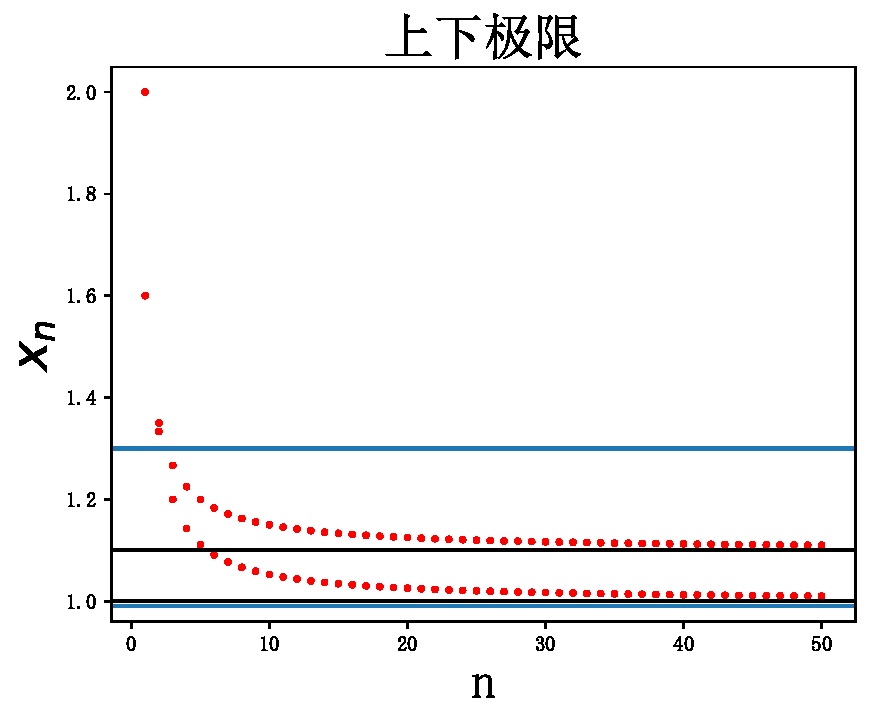
\includegraphics[scale=0.5]{tikz/上下极限散点图.pdf}
        \caption{上下极限散点图}
    \end{minipage}
    \vline
    \begin{minipage}[t]{0.5\linewidth}
        \vspace*{30pt}
        % 默认的行距是10pt
        所有都$\ge$
        $    
        \begin{cases}
            \Longrightarrow \text{里边最小的都}\ge\\ 
            \Longrightarrow \text{里边的最大的也}\ge 
        \end{cases}
        $

        \noindent
        $
        \begin{aligned}
            &\Longrightarrow x_n y_n \ge (H_1+\varepsilon)(H_2 + \varepsilon)\\ 
            &\Longrightarrow \lim_{n\to \infty}{x_ny_n} \ge \lim_{n\to \infty}{(H_1+\varepsilon)(H_2 + \varepsilon)}\\ 
            &\Longrightarrow \lim_{n\to \infty}{x_n y_n }\ge \lim_{n\to \infty}{x_n}\cdot \lim_{n\to \infty}{y_n}\\ 
            &\text{问题在哪里?}
        \end{aligned}
        $        
    \end{minipage}
    \end{figure}

   \subsection{内闭一致收敛}

   我们都知道函数列一致收敛的几何意义:就是当n充分大后的函数曲线系能够都落在关于极限函数的一个带形区域内(宽为2ε)。
   现在你要检查某个区间上函数列是否一致收敛,形象地讲,闭区间的端点就是你要考虑的范围、限度,
   出了这个界你就不考虑这个界以外的曲线能否落在你所预设好的带形区域内。那么,假设你已经知道在闭区间I上的某个函数列是内闭一致收敛的,
   并且很恰巧地你注意到n必须要非常非常大比如n=1000,你的这个函数列的曲线系才开始勉强落入带形区域。
   (这种极端情况正是接下来内闭一致收敛不是一致收敛的重要原因。)然后,你把闭区间I向外扩充一点点变成一个开区间D,于是,
   完全可能出现这样一种情况:n=1000已经不能让函数曲线们落入带形区间里了,你把n不断扩大,可是不管n怎么大,
   开区间的端点附近的x点总能找出一部分能让你的曲线系落到带形区间外,而且你没法定死最无法使你的曲线系落入带形区间的x点以便你能找到最大的n,
   因为这是开区间!端点处附近永远存在一部分点当你自以为找到足够大的n后让你的曲线系落到带形区间外。
   这就是某些内闭一致收敛不一定一致收敛例子的几何解释


   \subsection{同构的理解}
   \begin{figure}[!htb]
   \begin{minipage}[t]{0.5\linewidth}  
       如下图所示:
            \ctikzfig{tikz/Visaul_Mapping}
            \label{}
            \caption{映射关系图}
   \end{minipage}
   \hfill
   \begin{minipage}[t]{0.5\linewidth}
       若$\alpha = \beta + \gamma$ ,则$\sigma(\alpha + \beta) = \sigma(\gamma) = \sigma(\alpha) + \sigma(\beta)$

       \textbf{上式理解}\\
       \mycircled{1}$\alpha+\beta=\gamma\Rightarrow \sigma(\alpha)+\sigma(\beta)=\sigma(\gamma)$.(前面相等决定了后面一定相等)\\ 
       \mycircled{2}6因为是双射,所以我们也可以认为是$V'$中的每个元素都会被$V$中的元素所决\\ 
       \mycircled{3}我们把映射$\sigma$取逆,则可知:$V$中的每个元素被$V'$中的两个元素确定\\ 
       \mycircled{4}从2, 3点我们可以知道:$V$与$V'$中的对应元素的关系相同\\    
    \end{minipage}
    \end{figure}
    \begin{tcolorbox}[colback=blue!5!white,colframe=blue!75!black,title=线性空间的结构]
       所以我们可以认为线性空间的结构就是:\\ 
       \mycircled{1} 元素的个数\\ 
       \mycircled{2} 元素之间的关系(我们定义的加法和数乘)
       
       综上:

    $\sigma(\sigma^{-1})$的存在,使得$V(V')$中的元素均被$V'(V)$中的元素确定。确定了数乘与加法以及相同的元素个数,所以$\sigma (\sigma^{-1})$使得$V$与$V'$有了不同的结构。           
    \end{tcolorbox}


    \section{数学分析}
    \subsection{反三角函数的化解}  
    \begin{tcolorbox}[colback=blue!5!white,colframe=blue!75!black,title=反三角函数等式]
         \begin{equation}
            \arccos \frac{1}{x}=\operatorname{arcsec} x 
         \end{equation}
    \end{tcolorbox}     
    \begin{minipage}[b]{0.3\linewidth}
        \begin{align*}
            &\text{欲证:}  \arccos \frac{1}{x}=\operatorname{arcsec} x \\
            &\text{即证:}  \cos \left[\arccos \frac{1}{x}\right]=\cos [\operatorname{arcsec} x] \\
            &\text{即证:}  \frac{1}{x}=\cos [\operatorname{arcsec} x] \\
            &\text{另有}  \arctan x+\arctan \frac{1}{x}=\frac{\pi}{2} \Rightarrow x \in\left(0, \frac{\pi}{2}\right) 
        \end{align*}
        \end{minipage}
        \hfill
        \begin{minipage}[b]{0.3\linewidth}
        \ctikzfig{tikz/trangle}
    \end{minipage}
    \subsection{和差化积公式}
    \begin{tcolorbox}[colback=blue!5!white,colframe=blue!75!black,title=和差化积公式]
        \noindent{一些记号:余$\Longrightarrow$鱼(渔)}\\
        $\begin{array}{l|l}
                    \cos(\alpha)+\cos(\beta)=2\cos(\frac{\alpha+\beta}{2})\cos(\frac{\alpha-\beta}{2})&\hspace*{10em}\text{鱼 + 鱼 = 2条鱼}\nonumber \\
                    \cos(\alpha)-\cos(\beta)=-2\sin(\frac{\alpha+\beta}{2})\sin(\frac{\alpha-\beta}{2})&\hspace*{10em}\text{鱼 - 鱼=没有鱼}\nonumber \\\
                    \sin(\alpha)-\sin(\beta)=2\cos(\frac{\alpha+\beta}{2})\sin(\frac{\alpha-\beta}{2})&\hspace*{10em}\text{兄弟不和,渔翁得利}\nonumber \\
                    \sin(\alpha)+\sin(\beta)=2\sin(\frac{\alpha+\beta}{2})\cos(\frac{\alpha-\beta}{2})&\hspace*{10em}\text{兄弟相和,渔翁失利}\nonumber
                \end{array}$
    \end{tcolorbox}


    \section{和式}
    引入:看到一个双重求和的和式,但是我自己不会计算,很烦……
    \begin{align*}
        \sum _{i=0}^n \left[\sum _{j=1}^{n-i} j^2\right]=\frac{1}{12} n (n+1)^2 (n+2)
    \end{align*}
    
    \textbf{轮换求和与对称求和}

    两种形式
    \[\sum_{cyc}^{}{}\hspace*{0.5\linewidth}\sum_{ sym}^{}{}\]

    弄明白,尽量联系不等式里边的这两个东西。因为似乎在用了这个东西可以简化运算。

    \section*{求和符号基础知识}
    \textbf{对称式:}三元任意换仍未原式


    $x\Rightarrow y, y\Rightarrow z, z\Rightarrow x$.换完以后整体式子和原来恒等,比如$x+y+z, x^2 + y^2 + z^2, xy + yz + xz$ 

    \textbf{对称式:}依序(正反序)互换后仍为原式

    \subsection{常见的和式恒等变换}
    \begin{tcolorbox}[colback=blue!5!white,colframe=blue!75!black,title=和式恒等变换]
            \begin{align}
        &\left[
            \sum_{i=1}^{n}{a_i}
            \right]^2
            &=&
            \sum_{i=1}^{n}{a_i^2}
            +
            2\sum_{1 \le i \le i \le n}{a_i a_j}\nonumber\\
        &\left[
            \sum_{1 \le i \le i \le n}{(a_i - a_j)}
            \right]^2
            &=&
            n\sum_{i=1}^{n}{a_i^2}
            -
            \left[
            \sum_{i=1}^{n}{a_i}
            \right]^2\nonumber\\
        &\left[
            \sum_{i=1}^{n}{a_i}
            \right]
            \left[
            \sum_{i=1}^{n}{b_i}
            \right]
            &=&
            \sum_{i=1}^{n}{\sum_{j=1}^{n}{a_i b_j}}
             \quad = \quad
            \sum_{j=1}^{n}{\sum_{i=1}^{n}{a_i b_j}}\nonumber\\
        &\left[
            \sum_{1 \le i \le i \le n}{a_ia_j}
            \right]^2
            &=&
            \sum_{i=1}^{n}{\sum_{j=1}^{n}{a_i a_j}}
            \quad = \quad
            \sum_{j=1}^{n}{\sum_{i=1}^{n}{a_i b_j}}\nonumber\\
        &\sum_{i=1}^{n}{\sum_{j=1}^{n}{a_i a_j}}
            &=&
            \sum_{i=1}^{n}{a_i^2}
            +
            \frac{1}{2}
            \sum_{i=1}^{n}{\sum_{j=1}^{n}{[a_i b_j + a_j b_i]}}\nonumber\\
        &\sum_{i=1}^{n-1}{a_{i+1}-a_i}
            &=&
            a_n-a_1\nonumber\\
        &\sum_{i=1}^{n}{a_ib_i}
            &=&
            \sum_{i=1}^{n-1}{[(a_i-a_{i+1})B_i]}
            +a_nB_n\nonumber\\
        &\sum_{i=m}^{n}{a_ib_i}
            &=&
            \sum_{i=m}^{n-1}{[(a_i-a_{i+1})B_i]}
            +a_nB_n
            -a_mB_{m-1}\nonumber\\
        &\left[
            \sum_{i=1}^{n}{a_i^2}
            \right]
            \cdot 
            \left[
            \sum_{i=1}^{n}{b_i^2}
            \right]
            &=&
            \left[
            \sum_{i=1}^{n}{a_ib_i}
            \right]^2
            +
            \sum_{1\le i \le j \le n}({a_ib_j-a_jb_i})^2\nonumber
    \end{align}
    \end{tcolorbox}
    \subsection{预备准备}
    在证明之前,首先说明一个式子的几何意义,这对下面的证明有帮助
    $\sum\limits_{1 \leq i<j \leq n} a_{i} a_{j} $,它的几何意义如下边的左图\\
    \begin{figure}[!htb]
    \begin{minipage}{0.5\linewidth}
        \noindent
        $
            \sum\limits_{1 \leq i<j \leq n} a_{i j}=\\
            \left|\begin{array}{cccc}
            a_{1} a_{2} & +a_{1} a_{3} & & +a_{1} a_{n} \\
            +a_{2} a_{3} & \cdots & +a_{2} a_{n} & \\
            \vdots & \ldots & & \\
            +a_{n-1} a_{n} & & &\\
            \end{array}\right|\\
            \mbox{}\\
            \mbox{}\\
            \mbox{注:一共}(n-1)\mbox{行}(n-1)\mbox{列}
        $
    \end{minipage}
    \hfill
    \begin{minipage}{0.5\linewidth}
        \noindent
        $
            {A}=\left|\begin{array}{ccccc}
            a_{1} a_{1} & & & \cdots & \\
            a_{2} a_{1} & a_{2} a_{2} & \cdots & & \\
            \cdots & \cdots & a_{3} a_{3} & & \\
            a_{n-1} a_{1} & \cdots & \cdots & \cdots & \\
            a_{n} a_{1} & a_{n} a_{2} & \cdots & a_{n} a_{n-1} & a_{n} a_{n}
            \end{array}\right|
        $
    \end{minipage}
    \end{figure}
    \vspace{12pt}
    我们在这里引入另外一个记号,$A$,
    那么$A$旋转即可得到上边的$\sum\limits_{1 \leq i<j \leq n} a_{i j}$,其实$\sum\limits_{1 \leq i<j \leq n} a_{i j}$就是A的左下部分的旋转。
    \subsection{证明}
    \begin{figure}[!htb]
    \begin{minipage}[t]{0.5\linewidth}
    \textbf{(1)证明:}
    \begin{align}
        &\left(\sum\limits_{i=1}^{n} a_{i}\right)^{2}\nonumber\\
        &=\left(a_{1}+a_{2}+\cdots+a_{n-1}+a_{n}\right)^{2}\nonumber\\
        &=a_{1}\left(a_{1}+a_{2}+\cdots+a_{n-1}+a_{n}\right)\nonumber\\
        &+a_{2}\left(a_{1}+a_{2}+\cdots+a_{n-1}+a_{n}\right)\nonumber\\
        &+\cdots+a_{n}\left(a_{1}+a_{2}+\cdots+a_{n-1}+a_{n}\right)\nonumber\\
        &=\left|
        \begin{array}{ccccc}
            a_{1} a_{1} & +a_{1} a_{2} & +a_{1} a_{3} & \cdots & +a_{1} a_{n} \\
            +a_{2} a_{1} & +a_{2} a_{2} & \cdots & & \\
            \cdots & \cdots & +a_{3} a_{3} & & \\
            +a_{n-1} a_{1} & \cdots & \cdots & \cdots & \\
            +a_{n} a_{1} & +a_{n} a_{2} & \cdots & +a_{n} a_{n-1} & +a_{n} a_{n}
        \end{array}
        \right|\nonumber\\
        &=\sum\limits_{\mathrm{i}=1}^{\mathrm{n}} a_{\mathrm{i}}^{2}+2 \sum\limits_{1 \leq i<j \leq n} a_{i} a_{j}\nonumber\\
        &\Longrightarrow \text{注:第i行即第i项}\nonumber
    \end{align}
    \end{minipage}
    \vline
    \begin{minipage}[t]{0.5\linewidth}
    \textbf{(2)证明:}
    \begin{align}
        &\sum_{1 \leq i<j \leq n}^{n}\left(a_{i}-a_{j}\right)^{2}\nonumber\\
        &=\sum_{1 \leq i<j \leq n}^{n}\left(a_{i}^{2}-2 a_{i} a_{j}+a_{j}^{2}\right)\nonumber\\
        &=\left[\left(a_{1}^{2}-2 a_{1} a_{2}+a_{2}^{2}\right)+\cdots+\left(a_{1}^{2}-2 a_{1} a_{n}+a_{n}^{2}\right)\right]\nonumber\\
        &+\left[\left(a_{2}{ }^{2}-2 a_{2} a_{3}+a_{3}^{2}\right)+\cdots+\left(a_{2}{ }^{2}-2 a_{2} a_{n}+a_{n}{ }^{2}\right)\right]\nonumber\\
        &+\left[\left(a_{n-1}^{2}-2 a_{n-1} a_{n}+a_{n}^{2}\right)\right]\nonumber\\
        &=(n-1) \sum\limits_{i=1}^{n} a_{i}{ }^{2}-2\cdot
        \left|
        \begin{array}{cccc}
            a_{1} a_{2} & +a_{1} a_{3} & & +a_{1} a_{n} \\
            +a_{2} a_{3} & \cdots & +a_{2} a_{n} & \\
            \vdots & \ldots & & \\
            +a_{n-1} a_{n} & & &\\
        \end{array}
        \right|\nonumber\\
        &\begin{array}{l}
        =(n-1) \sum_{i=1}^{n} a_{i}{ }^{2}-2 \sum_{1 \leq i<j \leq n}^{n} a_{i} a_{j}
        \end{array}\nonumber\\
        &=n \sum_{i=1}^{n} a_{i}{ }^{2}-\left(\sum_{i=1}^{n} a_{i}{ }^{2}+2 \sum\limits_{1 \leq i<j \leq n}^{n} a_{i} a_{j}\right)\nonumber\\
        &\Longrightarrow \text { 由(1)易知 }\nonumber \\
        &=n \sum\limits_{i=1}^{n} a_{i}^{2}-\sum_{i=1}^{n} a_{i}^{2}\nonumber
    \end{align}
    \end{minipage}
    \end{figure}
   
    \noindent\rule{\textwidth}{1pt}\\
    \vspace{3pt}\\
    \textbf{(3证明:}
    \begin{align}
        \left[\sum_{i=1}^{n} a_{i}\right]\times\left[\sum_{j=1}^{n} b_{j}\right]
        &=\left|
        \begin{array}{ccccc}
            a_{1} b_{1} & +a_{1} b_{2} & +a_{1} b_{3} & \cdots & +a_{1} b_{n} \\
            +a_{2} b_{1} & +a_{2} b_{2} & \cdots & \\
            \cdots & \cdots & +a_{3} b_{3} & & \\
            +a_{n-1} b_{1} & \ldots & \cdots & \cdots & \\
            +a_{n} b_{1} & +a_{n} b_{2} & \cdots & +a_{n} b_{n-1} & +a_{n} b_{n}
        \end{array}\right| \nonumber\\
        &=a_{1} \sum_{j=1}^{n} b_{j}+a_{2} \sum_{j=1}^{n} b_{j}+\cdots+a_{n} \sum_{j=1}^{n} b_{j} \nonumber\\
        &=\sum_{i=1}^{n}\left[a_{i}\left(\sum_{j=1}^{n} b_{j}\right)\right]
        =\sum_{i=1}^{n}\left[\left(\sum_{j=1}^{n} a_{i} b_{j}\right)\right] \nonumber\\
        &=\sum_{i=1}^{n} \sum_{j=1}^{n} a_{i} b_{j}=\sum_{j=1}^{i \leftrightarrow j} \sum_{i=1}^{n} a_{j} b_{i} \nonumber\\
        &=\sum_{j=1}^{n} \sum_{i=1}^{n} a_{i} b_{j}\Longrightarrow\text { 此式说明多重求和时可以改变求和次序 }\nonumber
    \end{align}
    \clearpage
    \newpage
    \noindent\textbf{(4)证明:}\\
    \begin{figure}[!htb]
    \begin{minipage}{0.5\linewidth}
        \begin{align}
        &\sum\limits_{1 \leq i<j \leq n} a_{i j}=\nonumber\\
        &\left|
        \begin{array}{cccc}
            a_{1}a_{2} & +a_{1} a_{3} & & +a_{1} a_{n} \\
            +a_{2} a_{3} & \cdots & +a_{2} a_{n} & \\
            \vdots & \ldots & & \\
            +a_{n-1} a_{n} & & &\\
        \end{array}
        \right|\nonumber\\
        &=a_{1}\sum_{j=1+1}^{n} a_{j}+a_{2} \sum_{j=2+1}^{n} a_{j}+\cdots+a_{n-1} \sum_{j=(n-1)+1}^{n} a_{j}\nonumber\\
        &\Longrightarrow\mbox{以前标为基准, i为前标} \nonumber\\
        &=\sum_{i=1}^{n-1}\left[a_{i}\left(\sum_{j=i+1}^{n} a_{j}\right)\right] \nonumber\\
        &=\sum_{i=1}^{n-1}\left[\left(\sum_{j=i+1}^{n} a_{i} a_{j}\right)\right]\nonumber\\
        &=\sum_{i=1}^{n-1} \sum_{j=i+1}^{n} a_{i} a_{j}\nonumber\\
        &\mbox{以}45^{\circ}\mbox{线为行有:以斜标为基准,j为前标}\nonumber\\
        & =\left[a_{1}\right] a_{2}+\left[a_{1}+a_{2}\right] a_{3}+\cdots+\left[a_{1}+a_{2}+\cdots+a_{n-1}\right] a_{n} 
        \nonumber\\
        & =a_{2} \sum_{j=1}^{2-1} a_{j}+a_{3} \sum_{j=1}^{3-1} a_{j}+\cdots+a_{n}\sum_{j=1}^{n-1} a_{j} \nonumber
    \end{align}
    \end{minipage}
    \vline
    \begin{minipage}{0.5\linewidth}
        \begin{align}
        &=\sum_{i=2}^{n}\left[a_{i}\left(\sum_{j=1}^{i-1} a_{j}\right)\right] \nonumber\\
        &=\sum_{i=2}^{n}\left[\left(\sum_{j=1}^{i-1} a_{i} a_{j}\right)\right] \nonumber\\
        & =\sum_{i=2}^{n} \sum_{j=1}^{i-1} a_{i} a_{j} \nonumber\\
        &\Longrightarrow  \mbox{注:先取定外面的i值再展开内层}\nonumber\\
        &\mbox{若以后标为基准即有:}\nonumber\\
        &\mbox{若将方阵变化一下即有:}\nonumber\\
     LHS&=\left|
        \begin{array}{ccccc}
            +a_{1} a_{2} & +a_{2} a_{3} & +a_{3} a_{4} & \cdots & a_{n-1} a_{n} \\
            +a_{1} a_{3} & +a_{2} a_{4} & \vdots & \cdots& \\
            +a_{1} a_{4} & \vdots & +a_{3} a_{n} & & \\
            \vdots & +a_{2} a_{n} & & & \\
            +a_{1} a_{n} & & &
        \end{array}
        \right|\nonumber\\
        &\mbox{由对偶性知:}LHS=\sum_{j=1}^{n-1}\sum_{i=j+1}^{n}a_{i}a_{j}\nonumber\\
        &\mbox{综上:i, j只是一个记号而已}\nonumber
        \end{align}
    \end{minipage}
    \end{figure}
    % \noindent\makebox[\linewidth]{\rule{\paperwidth}{0.4pt}}
    \begin{figure}[!htb]
    \noindent\rule{\textwidth}{1pt}\\
    \vspace{3pt}\\
    \begin{minipage}[t]{0.3\linewidth}
        \textbf{(5)证明:}
        \begin{align}
        &=\frac{1}{2}\left(\sum_{{i}=1}^{{n}} \sum_{{j}=1}^{{n}} a_{{i}} {b}_{{j}}+\sum_{{i}=1}^{{n}} \sum_{{j}=1}^{{n}} a_{{i}} {b}_{{j}}\right) \nonumber\\
        &=\frac{1}{2} \sum_{{i}=1}^{{n}} \sum_{{j}=1}^{{n}}\left(a_{{i}} {b}_{{j}}+a_{{j}} {b}_{{i}}\right)\nonumber
        \end{align}
    \end{minipage}
    \hfill
    \begin{minipage}[t]{0.4\linewidth}
        \textbf{(6)证明:}
        \begin{align}
        &\sum_{i=1}^{n-1}\left(a_{i+1}-a_{i}\right)\nonumber \\
        &=\left(a_{2}-a_{1}\right)+\left(a_{3}-a_{2}\right)+\ldots+\left(a_{n}-a_{n-1}\right) \nonumber\\
        &=\left(a_{n}-a_{n-1}\right)+\ldots+\left(a_{3}-a_{2}\right)+\left(a_{2}-a_{1}\right) \nonumber\\
        &=a_{n}-a_{1}\Longrightarrow\mbox{此式即为伸缩求和}\nonumber
        \end{align}
    \end{minipage}
    \end{figure}
    \clearpage
    \newpage
    \noindent\textbf{(7)证明:}\\
    \noindent
    $
    \begin{aligned}
        & \mbox{首先把所有的}\mathrm{i}\rightarrow \mathrm{i}+1 \nonumber\mbox{于是有}n\to n-1\\
        & \sum_{i=2}^{n} A_{i-1} b_{i}=\sum_{i=1}^{n-1} A_{i} b_{i+1}\nonumber\\ 
        & \mbox{证法一:图解法,见陈纪修课本}\nonumber\\
    \end{aligned}
    $

    \begin{figure}[!htb]
    \begin{minipage}[t]{0.5\linewidth}
    \vspace{0pt}
    $    
    \begin{aligned}
        &\mbox{证法二:}\nonumber\\
        &\sum_{i=m}^{n} a_{i} b_{i} \nonumber\\
        &=\sum_{i=m}^{n}\left[\left(A_{i}-A_{i-1}\right) b_{i}\right] \nonumber\\
        &=\sum_{i=m}^{n} A_{i} b_{i}-\sum_{i=m}^{n} A_{i-1} b_{i} \nonumber\\
        &=\left(\sum_{i=m}^{n-1} A_{i} b_{i}+A_{n} b_{n}\right)-\sum_{i=m-1}^{n-1} A_{i} b_{i+1}\nonumber\\
        &\Longrightarrow\left\{\text { 把 } A_{i-1} \text { 变为 } A_{i} \text {, 方便后边提取公因式 }\right\} \nonumber\\
        &=\sum_{i=m}^{n-1} A_{i} b_{i}+A_{n} b_{n}-\left[\sum_{i=m}^{n-1} A_{i} b_{i+1}+A_{\mathrm{m}-1} b_{m}\right] \nonumber\\
        & \Longrightarrow\{\text { 把求和范围变为相同 }\} \nonumber\\
        & =\sum_{i=m}^{n-1}\left(A_{i} b_{i}-A_{i} b_{i+1}\right)+A_{n} b_{n}-A_{m-1} b_{m} \nonumber\\
        & =\sum_{i=m}^{n-1} A_{i}\left(b_{i}-b_{i+1}\right)+A_{n} b_{n}-A_{m-1} b_{m}\nonumber\\
        &\mbox{注: 此式即为Abel分部求和}\nonumber
    \end{aligned}
    $
    \end{minipage}
    \vline
    \begin{minipage}[t]{0.5\linewidth}
    \vspace{0pt} %不使用小页也能够对齐的。必须要在minnpage加上[t],而不是figure加[t] 
    \begin{align} 
        & \mbox{证法三:}\nonumber\\
        & \begin{aligned}
            &\sum_{i=1}^n a_i b_i \nonumber\\
            &=a_1 b_1+a_2 b_2+a_3 b_3+\cdots+a_n b_n \nonumber\\
            &=b_1\left(A_1-A_0\right)+b_2\left(A_2-A_1\right)\nonumber\\
            & ~+b_3\left(A_3-A_2\right)+\cdots+b_n\left(A_{n-1}-A_n\right) \nonumber\\
            &=\left(b_1-b_2\right) A_1+\left(b_2-b_3\right) A_2+\left(b_4-b_3\right) A_3\nonumber\\
            & ~+\cdots+\left(b_{n-1}-b_n\right) A_{n-1}+b_n A_n-b_1 A_0 \nonumber\\
            &=\sum_{i=1}^{n-1} A_i\left(b_i-b_{i+1}\right)+b_n A_n\nonumber
        \end{aligned}
    \end{align}
    \end{minipage}
    \end{figure}
    \begin{tcolorbox}[colback=blue!5!white,colframe=blue!75!black,title=Abel分部求和]
        \begin{align}
            \sum_{i=m}^{n}{a_ib_i}=\sum_{i=m}^{n-1} A_{i}\left(b_{i}-b_{i+1}\right)+A_{n} b_{n}-A_{m-1} b_{m}
        \end{align}
    \end{tcolorbox}
    \noindent\textbf{关于Abel分部求和公式的几点讨论}\\
    \mbox{}\\
    \noindent
    $
    \begin{aligned}
        &\langle 1\rangle\mbox{若定义}A_0=0\mbox{,那么当} m=1\mbox{时即有}\nonumber\\
        &\sum_{i=1}^n a_i b_i=\sum_{i=1}^{n-1} A_i\left(b_i-b_{i+1}\right)+A_n b_n\nonumber\\
        &\langle2\rangle\text{若}a_i\text{不便于求和,那么便有}\nonumber\\
        &\sum_{i=m}^n\left(A_i-A_{i-1}\right) b_i=\sum_{i=m}^{n-1} A_i\left(b_i-b_{i+1}\right)+A_n b_n-A_{\mathrm{m}-1} b_m\nonumber\\
        &\text{ 此式即为Abel和差变换}\nonumber\\
    \end{aligned}
    $

    \clearpage
    \newpage
    \noindent\textbf{(8)证明:}\\
    $
        \begin{aligned}
        &\left(\sum_{i=1}^n a_i^2\right)\left(\sum_{i=1}^n b_i^2\right)-\sum_{i=1}^n\left(a_i b_i\right)^2 \nonumber\\
        &=\sum_{i=1}^n \sum_{j=1}^n a_i^2 b_j^2-\sum_{i=1}^n \sum_{j=1}^n a_i b_i a_j b_j \nonumber\\
        &=\frac{1}{2} \sum_{i=1}^n \sum_{j=1}^n\left(a_i{ }^2 b_j^2-2 a_i b_i a_j b_j+a_j{ }^2 b_i{ }^2\right) \nonumber\\
        &=\frac{1}{2} \sum_{i=1}^n \sum_{j=1}^n\left(a_i b_j-a_j b_i\right)^2 \nonumber\\
        &=\sum_{1 \leq i<j \leq n}\left(a_i b_j-a_j b_i\right)^2\nonumber\\
        & \text{注:柯西不等式即证毕}\nonumber
        \end{aligned}
    $
    \begin{tcolorbox}[colback=blue!5!white,colframe=blue!75!black,title=拉格朗日恒等式]
        \begin{align}
            \left[
            \sum_{i=1}^{n}{a_i^2}
            \right]
            \cdot 
            \left[
            \sum_{i=1}^{n}{b_i^2}
            \right]
            &=
            \left[
            \sum_{i=1}^{n}{a_ib_i}
            \right]^2
            +
            \sum_{1\le i \le j \le n}({a_ib_j-a_jb_i})^2
        \end{align}
    \end{tcolorbox} 

    \section{三角函数两个和式的化解}
    这两个和式如下:
    \begin{tcolorbox}[colback=blue!5!white,colframe=blue!75!black,title=三角恒等式]
        \begin{flalign}
            &\sum_{k=1}^{n}{\sin(kx)}=\frac{\cos(n+\frac{1}{2})-\cos(\frac{x}{2})}{-2\sin(\frac{x}{2})}\nonumber\\
            &\sum_{k=1}^{n}{\cos(kx)}=\frac{\sin(n+\frac{1}{2})-\sin(\frac{x}{2})}{2\sin(\frac{x}{2})}
        \end{flalign}
    \end{tcolorbox}

    第一个式子的证明:
    \begin{align*}
        \sum_{k=1}^{n}{\sin(kx)}
        &=\frac{1}{\sin(\frac{x}{2})}[\sin(\frac{x}{2})\sin(x)+\sin(\frac{x}{2})\sin(2x)+\cdots+\sin(\frac{x}{2})\sin(nx)]\\
        &=\frac{1}{-2\sin(\frac{x}{2})}[[\cos(\frac{3x}{2})-\cos(\frac{x}{2})]+[\cos(\frac{5x}{2})-\cos(\frac{3x}{2})]+\cdots+[\cos(n+\frac{1}{2})x-\cos((n-\frac{1}{2})x)]]\\
        &=\frac{1}{-2\sin(\frac{x}{2})}[-\cos(\frac{x}{2})+\cos(n+\frac{1}{2})x]\\
        &=\frac{\cos(n+\frac{1}{2})x-\cos(\frac{x}{2})}{-2\sin(\frac{x}{2})}\\
        \mbox{证毕}
    \end{align*}
    第二个式子证明时,同样只需要乘以$\frac{1}{\sin(\frac{x}{2})}$
    \section{从定义上证明一个函数的可微性}
    \begin{align*}
        y=\sqrt[\frac{3}{2}]{x}
        \text{可以写成:}\Delta y = A \Delta x + o(\Delta x)
        \text{此时}A=\sqrt[\frac{3}{2}]{x}=\frac{3}{2}x^{-\frac{1}{3}}     
    \end{align*}
        \textbf{证明:}
    \begin{align}
    \Delta y&= \sqrt[3]{(x+\Delta x)^2} -\sqrt[3]{x^2}\notag \mbox{(想办法凑出}\frac{2}{3}x^{-\frac{1}{3}}\mbox{与}\Delta x)\\
        &= \frac{x+\Delta x}{\sqrt[3]{x+\Delta x}}-\frac{x}{\sqrt[3]{x}}\notag\\
        &= \frac{2}{3}\frac{\Delta x}{\sqrt[3]{x}}+\textcolor{blue}{\frac{1}{3}\frac{\Delta x}{\sqrt[3]{x}}+(x+\Delta x)(\frac{1}{\sqrt[3]{x+\Delta x}}-\frac{1}{\sqrt[3]{x}})}\notag\\
    \end{align}
    我们把(1)中的蓝色部分记作\ding{172},  %% \ding{}不能用在数学环境里边
意味着我们只需要证明
    
    \begin{equation}
        \lim_{\Delta x \rightarrow 0}\frac{\mycircled{1}}{\sqrt[3]{x}}=0
    \end{equation}  
    注:其实$\lim\limits_{\Delta x \rightarrow 0}{\frac{\frac{1}{\sqrt[3]{x+\Delta x}}-\frac{1}{\sqrt[3]{x}}}{\Delta x}}$就是求$\frac{1}{\sqrt[3]{x}} $的导数,
    求出(2)的极限即可:\\
    \textbf{证明:}

    \begin{align}
        \lim_{\Delta x \rightarrow 0}\frac{\mycircled{1}}{\sqrt[3]{x}}
        &=\lim\limits_{\Delta x \rightarrow 0}{\frac{\frac{1}{\sqrt[3]{x+\Delta x}}-\frac{1}{\sqrt[3]{x}}}{\Delta x}}\notag\\
        &=\frac{x}{\Delta x}\left( \frac{\frac{-\Delta x}{x\left( x+\Delta x \right) }}{\frac{1}{\sqrt[3]{\left( x+\Delta x \right) ^2} }+\frac{1}{\sqrt[3]{\left( x\left( x+\Delta x \right)  \right) } }+\frac{1}{\sqrt[3]{x^2} }} \right) \notag\\
        &=\frac{-\frac{x}{x^2}}{\frac{1}{3\sqrt[3]{x^2} }}\notag\\
        &=-\frac{1}{3}x^{-\frac{1}{3}}
    \end{align}
    总结:这里面主要就是用到公式$a^3-b^3=\left( a-b \right)\left( a^2+ab+b^2 \right)  $
    
    \section{二元函数中值定理的理解}
    \begin{align*}
     & f(a+h, b+k) - f(a, b) = f_x(a+\theta h, b + \theta k)h + f_y(a+\theta h, b + \theta k)k &\theta \in (0, 1)\\
     & \text{对比一元函数的拉格朗日中值定理:} \\
     & f(a+h) - f(a) = f_x(a+\theta h)h &\theta \in (0, 1)\\
    \end{align*}
    \section{Able判别法证明的一个反思}
    已知有Abel判别法和Dirichlet判别法:
    \begin{tcolorbox}[colback=blue!5!white,colframe=blue!75!black,title=Abel~Dirichlet判别法]
        \raggedright
        $
        \begin{aligned}
        &\sum_{n=1}^{\infty}{a_nb_n}\mbox{收敛,如果满足下列两个条件之一} \nonumber \\
        (1)&\{a_n\}\mbox{单调有界,}~\sum_{i=1}^{\infty}{b_i}\mbox{收敛} \\
        (2)& \{a_n\}\mbox{单调趋于0,}~\sum_{i=1}^{n}{b_i}\mbox{有界} \\
        \nonumber
        \end{aligned}
        $
    \end{tcolorbox}


    \subsection{错误的想法}
    设$\{a_n\}$有上界A ,$\sum\limits_{}^{\infty}{b_n}$收敛于C

    所以有$\sum\limits_{}^{\infty}{a_nb_n}<A \sum\limits_{}^{\infty}{b_n}=AC$


    错因分析: $\{b_n\}$不一定是正项级数,不能用比较判别法
    \subsection{正解}
    $
    \begin{aligned}
        &\sum_{}^{\infty}{a_n(B_n-B_{n-1})}\nonumber\\
        &=(a_1-a_2)B_1+\cdots+(a_n-a_{n-1})B_{n-1}+a_nB_n)\nonumber\\
        & \mbox{每一项都加绝对值有}\nonumber\\
        &=|\sum_{}^{\infty}{a_nb_n}|\nonumber\\
        & =|(a_1-a_2)B_1+\cdots+(a_n-a_{n-1})B_{n-1}+a_nB_n)|\nonumber\\
        & \mbox{设}|\sum_{\infty}^{b_n}|=A\nonumber\\
        & \mbox{于是有:}|\sum_{\infty}^{a_nb_n}|\ge A|(a_1-a_n)|+A|a_n|\nonumber\\
        & \ge (|a_1|+\cdots+ |a_n|)A\nonumber\\
        & =3\varepsilon A\nonumber
    \end{aligned}
    $
    \section{实数基本定理}
    \begin{questions}
    这六个定理虽然出发的角度不同,但是都是描述实数连续性这同一回事,他们之间是相互等价的,
    即任取其中两个定理,他们可以相互证明。他们在证明过程中相互联系。对同一个定理的证明,
    虽然不同的定理作为工具会使证明有简繁之分,有的用的是类似的证明方法,有的出发点与站的角度不同,
    但最后却能殊途同归。而有时使用同一个定理,也可能有不同的方法。即是方法相同,也有可能有不同的细节。
    作为工具,他们又各具特点。而这些都是值得我们去注意与发现的! 
    \end{questions}

    \noindent\ding{172} 确界存在定理:非空有上 (下)界数集,必有上 (下)确界。%英文字符和中文字符之间加一个空格不会警告

    \noindent\ding{173} 单调有界收敛原理:任何单调有界数列必有极限。

    \noindent\ding{174} 区间套定理:若$\{\left [ a_n,b_n \right ]\}$是一个区间套,则存在唯一一点$\xi$,使得$\xi\in \left [ a_n,b_n \right ] ,n=1,2,\cdots $

    \noindent\ding{175} \textit{Heine-Borel}有限覆盖定理:设$\left [ a,b \right ]$是一个闭区间,H为$\left [ a,b \right ]$的一个开覆盖,则在H中
    存在有限个开区间,它构成$\left [ a,b \right ]$上的一个覆盖。

    \noindent\ding{176} \textit{Weierstrass}聚点定理 (\textit{Bolzano}致密性定理:有界无穷数列必有收敛子列):直线上的有解无限点集至少有一个聚点。

    \noindent\ding{177} \textit{Cauchy}收敛准则:数列$\{a_n\}$收敛 $\Longleftrightarrow$对任给定的正数$\varepsilon$,总存在某一个自然数$N$,使得$\forall m,n>N$时,
    都有$\left | a_m-a_n \right|<\varepsilon\Longleftrightarrow\{a_n\}$是基本数列。
    

    \section{微分方程}
    \begin{tcolorbox}[colback=blue!5!white,colframe=blue!75!black,title=一阶线性微分方程的通解]
        $
         \begin{aligned}
              \mbox{标准形式}\frac{dy}{dx} + p(x)=q(x)&\nonumber\\
              &\hspace*{0.2\linewidth}\mbox{通解}y=e^{-\int_{}^{}{p(x)dx}}\cdot\int_{}^{}{[e^{\int_{}^{}{p(x) dx}} \cdot q(x)+C] dx}
        \end{aligned}
        $
    \end{tcolorbox}


    \noindent
    $
    \begin{aligned}
         \mbox{\textbf{证明:}}&\mbox{首先两边同时乘以积分因子}e^{\int_{}^{}{p(x) dx}}即有\nonumber \\
         \Longrightarrow&e^{\int_{}^{}{p(x) dx}}\cdot\frac{dy}{dx}+e^{\int_{}^{}{p(x) dx}}\cdot p(x)=q(x)\cdot e^{\int_{}^{}{p(x) dx}}\nonumber \\
         \Longrightarrow&\mbox{即有}\frac{d }{dx}[e^{\int_{}^{}{p(x) dx}}]=q(x)e^{\int_{}^{}{p(x) dx}}\nonumber \\
         \Longrightarrow &y=e^{-{\int_{}^{}{p(x) dx}}\cdot\int_{}^{}{e^{\int_{}^{}{p(x) dx}}\cdot q(x)dx}}\nonumber\\
         &\mbox{下边说明第一个积分}e^{\int_{}^{}{p(x) dx}}=\gamma(x).\mbox{不用+任意常数C}\\
         &\mbox{假设}e^{\int_{}^{}{p(x) dx}}=\gamma(x)+C\nonumber\\
         &\mbox{带入上边的式子即有}\nonumber\\
         &y=e^{-\gamma(x)-C}\cdot \int_{}^{}{e^{\gamma(x)+C}\cdot q(x) dx}\nonumber\\
         \Longrightarrow  &y=e^{-C}\cdot e^{-\gamma(x)}\cdot e^C\cdot \int_{}^{}{e^{\gamma(x)}\cdot q(x)dx}\nonumber\\
         \Longrightarrow &y=e^{-\gamma(x)}\cdot\int_{}^{}{e^{\gamma(x)}\cdot q(x)dx}\nonumber\\
     \end{aligned} 
    $

    \noindent{所以从上边我们可以看出,第一个积分可以不加常数C}\\
    但是注意:上边只是非齐次方程的特解, 我们还应该加上齐次方程的通解。
    所以可以得到原微分方程的通解为:
         \begin{align}
             y=e^{-\int_{}^{}{p(x)dx}}\cdot\int_{}^{}{[e^{\int_{}^{}{p(x) dx}} \cdot q(x)+C] dx}\nonumber
         \end{align}
    \subsection{两个错误的带入公式的例子}
    \begin{figure}[!htb]
    \begin{minipage}[t]{0.5\linewidth}
        \vspace*{2pt}
        \noindent
        $
            \begin{aligned}
                &xy'+(x+1)y=e^x\\
                &\mbox{先求出齐次方程的通解}y=e^{\int_{}^{}{\frac{1+x}{x} dx}}\\
                \Longrightarrow& \mbox{原来非齐次方程的解即为:}\\
                y&=e^{\int_{}^{}{\frac{1+x}{x} dx}}[\int_{}^{}{e^{\int_{}^{}{\frac{1+x}{x} dx}}\cdot \frac{e^x}{x} dx}]\\
                &=e^{\ln |x|+x}[\int_{}^{}{e^{\ln |x|+x} \cdot \frac{e^x} {x}dx}]\\
                &=|x|e^x[\int_{}^{}{e^{2x} dx}]\\
                &=xe^x\cdot(\frac{1}{2}e^{2x}+C)
            \end{aligned}
        $

        \textcolor{blue}{错因:积分因子乘过去没有取倒数}
    \end{minipage}
    \hfill
    \begin{minipage}[t]{0.5\linewidth}
        \vspace*{2pt}
        \noindent
        $
            \begin{aligned}
                &\text{首先求得:积分因子}=e^{\int_{}^{}{\frac{x+1}{x} dx}}=xe^x\nonumber \\
                &\text{然后使用公式可以知道:}y=\frac{1}{xe^x}\cdot \int_{}^{}{e^x\cdot xe^x dx}\nonumber \\
                &\Longrightarrow y = \frac{e^{-x}}{x}\cdot (\frac{1}{2}xe^x-\frac{1}{4}e^{2x}+C)\nonumber \\
                &\Longrightarrow y = (\frac{1}{2}-\frac{1}{2x})e^x + C\cdot \frac{e^{-x}}{x}\nonumber
            \end{aligned} 
        $
        \vspace*{4pt}

        \textcolor{blue}{错因:原方程两边同时除以}$x$\textcolor{blue}{时没有对右边的}$e^x$\textcolor{blue}{除以}$x$.

        正解: 只需要把第二种错误的解法稍微改善以下就可以得到正解
        \begin{tcolorbox}[colback=blue!5!white,colframe=blue!75!black,title=]
            \[
                y = \frac{e^x}{2x}+C\frac{e^{-x}}{x}
            \]
        \end{tcolorbox}  
    \end{minipage}
    \end{figure}
    \newpage
    \begin{figure}[!htb]
        \begin{minipage}[t]{0.5\linewidth}
            \vspace*{1em}
            \noindent$
            \begin{aligned}
                & \textbf{求解如下的二阶微分方程}\\
                &x'' -x = C_0 \\
                &x'' - x' + x' - x = 0 \\
                &g'(t) - g'(t)=C_0\hspace*{2em} \textbf{其中:} g(t) = x'(t) -x(t) \\
                &\Longrightarrow \textbf{验证可得:} g(t) = -C_0 + ce^{-t}\\
                &\textbf{验证:}g'(t) - g(t) = ce^{-t} -(-C_0 + ce^{-t}) = C_0\\
                &\textbf{然后求解:}x'(t) - x(t) = ce^{-t} -C_0\\
            \end{aligned} 
            $
        \end{minipage}
        \begin{minipage}[t]{0.5\linewidth}
            \vspace*{1em}
            \noindent$
            \begin{aligned}
                &\textbf{但是如果直接代入公式是得不到正确的}g(t)\textbf{的}\nonumber \\
                g(t) &= e^{-\int_{}^{}{-1}dt}\cdot \int_{}^{}{e^{\int_{}^{}{-1}}dt} \nonumber \\
                &= C_0 e^{t} (e^{-t}+e^{c_1})\nonumber \\
                &= C_0 + e^{c_1}\cdot C_0  e^t\\
                &= C_0 + Ce^t
            \end{aligned} 
            $
        \end{minipage}
    \end{figure}

    \section{恰当微分方程}
    已知有方程
    \begin{align}
             (2x + \frac{1}{y}) dx  + (\frac{1}{y^2}-\frac{x}{y^2})dy=0\nonumber
    \end{align}
    \subsection{分项组合}
    \[\frac{1}{y}dx -\frac{x}{y^2}dy=d\frac{x}{y}+xd\frac{1}{y}=2\cdot d\frac{x}{y}\] 

    当时的错误想法:认为y与x无关,那么在$\frac{1}{y}dx$中,$\frac{1}{y}$就时一个常数,常数当然可以拿到微分后边去。
    所以后边$\frac{x}{y^2}dy$当然也同理,认为x与y没有关系。于是就产生了这个错误。

    \textcolor{blue}{错因:认为$x$与$y$无关,他们都有微分方程了,那么就可以认为$y=y(x)$的了,必然二者有关系。也就是说$x$不能随便的放到后边的$dy$中了。}

    \textbf{反思}

    今后$f(x)dx$可以把f(x)做一个积分,然后放到$dx$里边去,$f(y)dy$类似,但是遇到形如$f(x)dy \text{或}f(y)dx$的东西的时候一定要找前后的搭配。

    \textbf{常见的凑微分形式}

    \begin{tcolorbox}[colback=blue!5!white,colframe=blue!75!black,title=常见的凑微分形式]
    \noindent
    $
        \begin{aligned}
            &xdy + ydx = d(xy) \hspace*{0.3\linewidth}  & \frac{ydx-xdy}{y^2}=d(\frac{x}{y})\nonumber \\
            &\frac{ydx -xy}{xdy}=d[\ln(\frac{x}{y})] & \frac{ydx-xdy}{x^2+y^2}=d[arccot(\frac{y}{x})]\nonumber\\
            &\frac{ydx-xdy}{x^2-y^2}=\frac{1}{2}d[\ln|\frac{x-y}{y-x}|]&~~\nonumber
        \end{aligned}  
    $
      
    \end{tcolorbox}
    
    \subsection{曲线积分}
    因为已知有:$u(x,y)=\int_{x_0}^{x}{M(x,y_0) dx}+\int_{y_0}^{y}{N(x,y) dy}$.
    于是我们取点$(x_0,y_0)=(0, 1)$,带入上边即有:\\
    \begin{figure}[!htb]
    \begin{minipage}[t]{0.4\linewidth}
    \hspace*{1pt}

    $
    \begin{aligned}
    u(x,y)&=\int_{0}^{x}{M(x,1) dx}+\int_{1}^{y}{N(x,y) dx}\nonumber\\
        &=\int_{0}^{x}{2x+1 dx}+\int_{1}^{y}{[\frac{1}{y}-\frac{x}{y^2}] dy}\nonumber\\
        &=x^2+x+C_1+\ln|y|+\frac{x}{y}+C_2\nonumber\\
        &\text{所以最终可以知道}\nonumber\\
        &u(x,y)=x^2+x+\ln|y|+\frac{x}{y}+C\nonumber
    \end{aligned}
    $
    \end{minipage}
    \begin{minipage}[t]{0.2\linewidth}
    \centering
        \color{blue}{$\Longrightarrow$}
    \end{minipage}
    \begin{minipage}[t]{0.4\linewidth}
    \hspace*{1pt}

    \color{blue}
    {
        错因:\\
        在$\int_{1}^{y}{\frac{1}{y}-\frac{x}{y^2}}dy$中,当$y=1$时,有一个$\frac{1}{1}-\frac{x}{1}=1-x$.但是我们忽略了它。


    }
    \end{minipage}
    \end{figure}

    \noindent\textbf{老师的正解:}

    首先判断该方程是否为恰当微分方程,有$\frac{\partial M}{\partial y}=\frac{-1}{y}=\frac{\partial N}{\partial x}$,所以该方程是一个恰当的微分方程。同时取点$(0, 1)$,于是就可以得到:\\
    \vspace*{3pt}\\
    $
        \begin{aligned}
            u(x,y)&=\int_{0}^{x}{\frac{2xy+1}{y}+\int_{1}^{y}{\frac{y-0}{y^2} dx} dx}\nonumber \\
            &=x^2+\frac{x}{y}+\ln|y||_1^y\nonumber \\
            &=x^2+\frac{x}{y}+\ln|y|+C\nonumber \\
        \end{aligned} 
    $

    \textbf{曲线积分方法}

    \begin{tcolorbox}[colback=blue!5!white,colframe=blue!75!black,title=曲线积分法]
    $
        \begin{aligned}
            \text{标准形式:}M(x,y)dx+N(x,y)dy=\frac{\partial u}{\partial x}dx&+\frac{\partial u}{\partial y}dy\\
            &\text{标准解1:}u(x,y)=\int_{x_0}^{x}{M(x,y_0) dx} + \int_{y_0}^{y}{N(x,y) dy}\\
            &\text{标准解2:}u(x,y)=\int_{y_0}^{y}{N(x_0,y) dy} + \int_{x_0}^{x}{M(x,y) dx}\\
        \end{aligned}
    $ 

    \textbf{理解}


    ~~~~我们可以认为是先从$(x_0, y_0)\to(x, y_0)$积分,因为此时只有x在变化,y是常数,恒为$y_0$,所以这个值就是$\frac{\partial }{\partial x}\int_{y_0}^{y}{M(x,y_0) dy}$.
    然后第二项就是从$(x, y_0)\to (x, y)$,此时只有y在变化,x为常数,恒为$x$,所以第二项就是$\int_{y_0}^{y}{N(x, y) dx}$.

    所以综上我们就可以得到:

    \[
        u(x,y)=\int_{x_0}^{x}{M(x,y_0) dx} + \int_{y_0}^{y}{N(x,y) dy}\nonumber
    \]
    \end{tcolorbox}

    \textbf{曲线积分方法的证明}

    我们从$\frac{\partial u}{\partial y}=N(x,y)$入手。

    $
        \begin{aligned}
            u(x,y)&=\int_{y_0}^{y}{N(x,y) dy}+\psi(x)\nonumber \\
            &\Longrightarrow \frac{\partial}{\partial x}[\int_{y_0}^{y}{N(x,y) dy}]+\psi'(x)=M(x,y)\nonumber \\
            &\Longrightarrow \psi'(x)=M(x,y)-\frac{\partial}{\partial x}[\int_{y_0}^{y}{N(x,y) dy}]+\psi'(x)\nonumber \\
            &=M(x,y)-\int_{y_0}^{y}{\frac{\partial}{\partial x}N(x,y) dy}\nonumber\\
            &=M(x,y)-\int_{y_0}^{y}{M(x,y) dy}\nonumber\\
            &=M(x, y)-[M(x,y)-M(x,y_0)]\nonumber\\
            &\text{带入最上边的式子即可的得:}\nonumber\\
            &\Longrightarrow u(x,y)=\int_{y_0}^{y}{N(x,y) dy}+\int_{x_0}^{x}{M(x,y_0) dx}
        \end{aligned} 
    $

    \textbf{错误的简单记忆方式}

    $
        \begin{aligned}
            u(x,y)&=\int_{}^{}{M(x,y_0) dx}+\int_{}^{}{N(x,y) dy}\nonumber \\
            &=\int_{}^{}{M(x,y) dx}+\int_{}^{}{N(x,y_0) dy}\nonumber \\
        \end{aligned} 
    $

    正确性有待检验$\cdots$

    \textcolor{blue}{这种记忆方法完全是错的,就像上边的错误1,这样会漏掉常数项对应的$x,y$的多项式。}
    \subsection{判定定理}
    \begin{tcolorbox}[colback=blue!5!white,colframe=blue!75!black,title=判定定理]
    \begin{align}   
       u(x, y) = \int_{}^{}{M(x, y) dx} + \int_{}^{}{[N(x, y)-\frac{\partial}{\partial y}\int_{}^{}{M(x, y) dx}] dy}\nonumber 
    \end{align}         
    \end{tcolorbox} 
    

    \subsection{积分因子}
    作用:把非恰当的微分方程转化为恰当的微分方程
    
    \textbf{引入}

    $xdy-ydx=0$,很容易看出这不是一个恰当微分方程,因为$\frac{\partial M(x, y)}{\partial y}=-1\neq \frac{\partial N(x, y)}{\partial x}=1$。这个时候我们在两边同时乘以$\frac{1}{y^2}$就可以得到:$\frac{1}{y}dx-\frac{x}{y^2}dy=0$.即$d(\frac{x}{y})=0\Longrightarrow \frac{x}{y}=C$。

    关于怎么凑积分因子:可以记住常见的二元函数的微分形式。见前面的常见的\textbf{常见的凑微分形式}。

    \textbf{积分因子的推导}

    背景:如果存在连续可微的函数$u(x, y)$,使得 
    \begin{align}
        &u(x, y)M(x, y)dx + u(x, y)N(x, y)dy=0\nonumber
    \end{align}
    恰好为恰当微分方程。则称$u(x, y)$为方程的积分因子。

    根据恰当微分方程的判定定理可以知道,函数$u(x, y)$为不恰当微分方程的解的\textbf{充要条件}为:
    \begin{align}
        &\frac{\partial (\mu M)}{\partial y}=\frac{\partial (\mu N)}{\partial x}\nonumber\\
        \Longrightarrow& N  \cdot \frac{\partial \mu}{\partial x}-M\cdot \frac{\partial \mu}{\partial y} = [\frac{\partial M}{\partial x} - \frac{\partial N}{\partial x}]\nonumber\\
        &\text{这是一个一阶偏微分方程, 直接求解$\mu(x, y)$是很复杂的。所以我们一般考虑积分因子为单变量函数的情形。}\nonumber\\
        \Longrightarrow& \text{即}\mu= \mu(x)\text{或}\mu = \mu(y)\text{如果$\mu$只与x(y同理)有关,那么就有} \frac{\partial \mu}{\partial y}=0.\nonumber\\
        \Longrightarrow& \text{原来的偏微分方程就可以简化为:}N\cdot \frac{d\mu}{d x} = [\frac{\partial M}{\partial y}-\frac{\partial N}{\partial x}]\cdot\mu\nonumber\\
        \Longrightarrow&\frac{d\mu}{\mu} = \frac{\frac{\partial M}{\partial y}-\frac{\partial N}{\partial x}}{N}
        dx\nonumber\\
        \Longrightarrow& \text{得出一个结论}\frac{\frac{\partial M}{\partial y}-\frac{\partial N}{\partial x}}{N}=\psi(x)\nonumber\\
        \Longrightarrow& \mu (x) = e^{\int_{}^{}{\psi (x) dx}}\nonumber
    \end{align}

    \begin{tcolorbox}[colback=blue!5!white,colframe=blue!75!black,title=积分因子的寻找方法] 
    只需要去尝试以下的两个式子即可,看能否只和一个变量有关

    \vspace{3pt}

    $
    \begin{aligned}
        \frac{\frac{\partial M}{\partial y}-\frac{\partial N}{\partial x}}{N}=\psi(x) \hspace*{0.6\linewidth} \frac{\frac{\partial M}{\partial y}-\frac{\partial M}{\partial x}}{-M}=\varphi(x)\nonumber
     \end{aligned} 
    $

     \end{tcolorbox}

     \subsection{一阶隐式微分方程}
     一阶隐式微分方程的一般形式为
     \begin{align}
         F(x, y, y') = 0\nonumber
     \end{align}
     但是有一般形式的隐式方程解决的难度过大,且没有通用的解决方法。于是下边主要针对它化简为的4种形式进行讨论。
     
     $
     \begin{array}{cccc}
        y = f(x, y') & y = f(y, y')& F(x, y')= 0; & F(y, y')= 0
     \end{array}
     $

     首先申明一个点,其实上边只有两种情况,毕竟$x, y$是等价的。

     \textbf{第一种形式的求解}

     令 $y' = p$, 从而就有$\frac{\partial y}{\partial x} = \frac{\partial }{\partial x}f(y, p)$, 从而就有
     $p = \frac{\partial f}{\partial x}+\frac{\partial f}{\partial p}\frac{dp}{dx}$,然后就可以得到$\Phi(x, p, c)=0$。从而方程的解为
     \[\begin{cases}
         &\Phi(x, p, c) = 0\\
         &y = f(x, p)
     \end{cases}\]

     \textcolor{blue}{注意:$f(x, p)$一定要使用多元函数求导法则进行求导。}

     \textbf{第二种形式的求解}
     也就是形如$F(x, y')= 0$的方程的求解。和第一种思想相似,也是令$y'=  p$,所以就有$F(x, p) = 0 $。从几何意义上说它就是平面$Oxp$上的一条曲线, 所以它不然可以用一个如此下的参数方程表示:
     \[\begin{cases}
         &x = \varphi(t)\\
         &p = \psi(t)
     \end{cases}\]
     从参数方程的求导法则可以知道,
     \begin{align*}
     \frac{dy}{dx}& = \frac{\frac{dy}{dt}} {\frac{dx}{dt}} = p  \\
                \Longrightarrow  \frac{dy }{dt } &= p\cdot \frac{dx }{dt } = \psi(t) \varphi'(t)\\
                \Longrightarrow  y &= \int_{}^{}{\psi (t ) \varphi' (t)dt}
     \end{align*}



   \textbf{ 一个具体的例子}

   解方程 $x^3 + y'^3 - 3 xy'= 0$.其中$\frac{dy }{dx }$\\
   \textbf{解:}

   \begin{align*}
    \Longrightarrow &\text{首先令}y' = p = tx,\text{带入原始的中得}\\ 
    \Longrightarrow & \text{\textcolor{blue}{备注:这里实际上是设$x =  x(t)\to  y = t\cdot x(t) \to y = y(t)$}}\\
    &x = \frac{3t }{1+t^3} \Longrightarrow p = \frac{3t^2}{ 1+t^3}\\ 
      \Longrightarrow & \text{\textcolor{blue}{
       备注:这里不能认为$y = \int_{}^{}{p  dt}$,因为我们求的是$y=y(t)$ 但是这里是$ y = y(t)$.
       }}\\ 
    &\text{\textcolor{blue}{
        ~~~~~~~也就更谈不上把$y = y(t)$解出来以后,反解$t = t(x)$带入$p = \frac{3t^2}{1+t^3}$从而得到$y = y(x)$了
        }}\\
    & dy = \frac{9(1-2t^3)t^2}{(1+t^3)^3}dt\\
    & \text{\textcolor{blue}{
    备注:这里就是得到$y = y(t)$的表达式。因为前边$x= x(t)$的表达式也求出来了}}\\ 
    \Longrightarrow & \text{积分可得:} y = \int_{}^{}{\frac{9(1-2t^3)t^2}{(1+t^3)^3} dt} = \frac{3}{2}\cdot \frac{1+4t^3}{(1+t^3)^2} + C
   \end{align*}

   ~~~~原方程的解为:
   \[\begin{cases}
      & x= \frac{3t }{1+t^3}\\ 
      & y = \frac{3}{2}\cdot \frac{1+4t^3}{(1+t^3)^2} + C
   \end{cases}\]

   \newpage
   \noindent\textbf{积分因子}

   试证明\textbf{齐次}微分方程$M(x, y)dx + N(x, y)dy = 0$,当$xM + yN \neq 0$时有积分因子:$ \mu = \frac{1}{xM + y N}$

   \noindent\text{自己的做法:}

   \vspace*{1em}
   \noindent\textbf{证明:}

   \vspace*{1em}
   \noindent$
    \begin{aligned}
        &\frac{\partial }{\partial y}\frac{M}{xM+yN}=\frac{\partial }{\partial x}\frac{N}{xM+yN}\\
        &L H S=\frac{\partial}{\partial y}\left(\frac{M}{x M+y N}\right)=\frac{M_y(x M+y N)-\left(x M_y+N+y N_y\right) \cdot M}{(x M+y N)^2}\\
        &\text { RHS }=\frac{\partial}{\partial x}\left(\frac{N}{x M+y}\right)=\frac{N_x(x M+y N)-\left(M+x M_x+y N_x\right)\cdot N}{(x M+y N)^2}\\
    \end{aligned}
    $

    \vspace*{1em}
    \noindent$\text{ 即证: } M_y(x M+y N)-\left(x M_y+N+y N_y\right) \cdot M=N_x(x M+y N)-\left(M+x M_x+y N_x\right) \cdot N$
    
    \noindent$
    \begin{aligned}
        (M_y-N_x)(x M+y N)&=M(x M_y+N+y N_y)-N\cdot(M+x M_x+y N_x)\\
        &=M x \cdot M_y+{M N}+y M N_y-{N M}-x N M_x-y N N_x\\
        &=M x \cdot M_y+y M N_y-x N M_x-y N N_x\\
        & = RHS
    \end{aligned}
    $
    
    \noindent $
    \Longrightarrow L H S= \cancel {x M M_y} - \cancel{y N N_x} + y N M_y - x M N_x = \cancel{ x M \cdot M_y} + y M N_y-x N M_x- \cancel{y N N_x} = RHS
    $

    \noindent$
    \begin{aligned}
        &\text {即证:} y N M_y - x M N_x = y M N_y - x N M_x\\
        &\text{以下就是两个思考方向:}\\
        &\Rightarrow 1^0 \quad y(N\cdot M_y - M\cdot N_y) = x(M\cdot N_x - N\cdot M_x)\\
        &\Rightarrow 2^0 \quad M\left(x N_x+y N_y\right)=N\left(x M_x+y M_y\right)
    \end{aligned}
    $
    
    \vspace*{1em}
    \noindent\textbf{背景知识补充}

    \begin{tcolorbox}[colback=blue!5!white,colframe=blue!75!black,title=齐次函数]
     \noindent \textbf{定义}

     如果把函数$f(x_1, x_2, \cdots , x_n)$的每一个自变量乘以一个因子$\lambda$, 如果此时因变量相当于原函数
     乘以这个因子$\lambda$的幂,则称此函数为齐次函数。
     定义$f(x_1, x_2, \cdots , x_n)$为$k$次齐次函数,需满足关系:
     \begin{align*}
      f(\lambda x_1, \lambda x_2, \cdots , \lambda x_n) = \lambda^{k} f(x_1, x_2, \cdots , x_n)
     \end{align*} 

     \noindent \textbf{欧拉定理}

     对于$k$次齐次函数$f(x_1, x_2, \cdots , x_n)$, 有齐次函数的欧拉定理:
     \begin{align}
      x_1 \frac{\partial f}{\partial x_1} + x_2 \frac{\partial f}{\partial x_2} + \cdots + x_n \frac{\partial f}{\partial x_n} = kf(x_1, x_2, \cdots , x_n)
    \end{align}
    \noindent\textbf{齐次方程}

    如果方程
    \[\frac{dy}{dx}= f(x, y)\]
    的右端函数$f(x, y)$为它的变量的\textbf{零次}齐次函数,即满足恒等式
    \[f(tx, ty) = f(x, y)\]
    那么上述方程称为齐次方程.
    \end{tcolorbox}
    \newpage
    \begin{figure}[!htb]
        \begin{minipage}[t]{0.5\linewidth}
            \noindent\textbf{欧拉定理的证明}

            \vspace*{1em}
            因为函数$f(x_1, x_2, \cdots , x_n)$为$k$次齐次函数, 所以对定义式两边全微分有:
       
            \noindent
            $
            \begin{aligned}
               \frac{\partial }{\partial \lambda} LHS 
                   & =\frac{d}{d\lambda}f(\lambda x_1, \lambda x_2, \cdots , \lambda x_n) \\
                   & = \sum_{i=1}^{n}{\frac{\partial f}{\partial (\lambda x_i)}\frac{d (\lambda x_i)}{d \lambda}}\ \\
                   & = \sum_{i=1}^{n}{x_i \frac{\partial f}{\partial (\lambda x_i)}} \\
                   & = \frac{\partial }{\partial \lambda} RHS \\
                   & = \frac{d}{d \lambda} \lambda^k f( x_1,  x_2, \cdots ,  x_n) \\
                   & = k \lambda^{k-1}f( x_1,  x_2, \cdots ,  x_n)\\
                   \Longrightarrow &\sum_{i=1}^{n}{x_i \frac{\partial f}{\partial (\lambda x_i)}}  = k \lambda^{k-1}f( x_1,  x_2, \cdots ,  x_n)\\
            \end{aligned} 
            $
       
            $
            \begin{aligned}
               \text{令} \lambda = 1, \text{我们即有}
               \sum_{i=1}^{n}{x_i \frac{\partial f}{\partial (x_i)}} & = k f( x_1,  x_2, \cdots ,  x_n)
            \end{aligned} 
            $
        
        \end{minipage}
    \vline
        \begin{minipage}[t]{0.5\linewidth}
            \noindent\textbf{齐次多项式}
            
            \vspace*{1em}
            由同次数的单项式相加得到的多项式。\\比如$x^5 + 2x^3y^2 + 9x*4y - 4 y^5$是5次齐次多项式(函数)
        \end{minipage}
    \end{figure}

    \vspace*{2em}
    \noindent{上述自己的解法(思考方向$1^\circ$)完善}
    \[LSH = k M N(x, y) = k M(x, y) N = RSH, ~~~ k = 1\]

    \vspace*{2em}
    \noindent\textbf{参考证明:}\\
    \vspace*{1em}

    $
    \begin{aligned}
        &\text{设}M(x, y), N(x, y)\text{是}m\text{次齐次函数, 令}y = ux, u = u(x) \rightarrow dy = xdu + u dx\\
        &M(x, y) = M (x, ux) = x^m M(x, y)\\
        &N(x, y) = N (x, ux) = x^m N(x, y)\\
        &\text{方程两边同时乘以乘积因子} \mu  = \frac{1}{xM +yN}(xM + yN \neq 0)\text{得:}\\
        &\hspace*{6em}\frac{M}{xM + yN} dx + \frac{N}{xM + yN}dy =0\\
        &\text{把}dy \to xd\mu  + \mu dx\text{即有:}\\
        &\hspace*{4em}\frac{M(x,\mu)+ \mu N(x, \mu x)}{xM(x, \mu x)+ yN(x, \mu x)}dx + \frac{xN(x, \mu x)}{xM(x, \mu x)+ yN(x, \mu x)}d\mu = 0\\
        &\text{展开化解:}\frac{x^m M(1, \mu)+ ux^m N(1, \mu)}{x^{m+1} M(1, \mu)+ ux^{m+1} N(1, \mu)}dx + \frac{x^{m +1} N(1, \mu )}{x^{m+1} M(1, \mu)+ ux^{m+1} N(1, \mu )}d\mu = 0\\
        & \text{化简即得:}\frac{1}{x}dx + \frac{N(1, \mu)}{M(1, \mu)+ \mu N(1, \mu)}d \mu = 0\\
        &\text{进行恰当微分方程得检验可知:} \frac{\partial }{\partial \mu} \left[\frac{1}{x}\right] = 0 = \frac{\partial }{\partial x}\left[\frac{N(1, \mu)}{M(1, \mu)+ \mu N(1, \mu)}\right]\\
        & \text{故上述方程为恰当微分方程} \Rightarrow \mu  = \frac{1}{xM +yN}(xM + yN \neq 0)\text{是积分因子}
    \end{aligned} 
    $

    从上边的解答过程中还可以得到方程: 
    \[M(x, y)dx + N(x, y)dy=0, (xM+ yN \neq 0)\]
    的解为:
    \[x = ce^{-\int_{}^{}{\frac{N(1, \mu)}{M(1, \mu)+ \mu N(1, \mu)}d \mu}}\]
    提示: 
    \[
        \frac{1}{x}dx + \frac{N(1, \mu)}{M(1, \mu)+ \mu N(1, \mu)}d \mu = d\left[\frac{1}{x}\right] + d\left[\int_{}^{}{\frac{N(1, \mu)}{M(1, \mu)+ \mu N(1, \mu)} d \mu}\right] = 0
    \]
    \vspace*{2em}
   \noindent\textbf{皮卡逼近}

   已知有方程
   \[
        \frac{dy}{dx}=y, y(0)=1
    \]
   若$,y=y(x)$是原微分方程的解,带如上述方程有
   \[dy(x)=y(x)dx\]
   \textbf{然后两边积分有:}
   \[y(x)=\int_{0}^{x}{y(s) ds}\]
   反之,我们可以得到:若一个连续函数满足上述的积分方程,那么它就是上述的微分方程的解


    \section{使用定义求取黎曼积分}
        \begin{tcolorbox}[colback=blue!5!white,colframe=blue!75!black, title=黎曼和的定义]
            设$f(x)$是定义在$[a,b]$上的有界函数,在$[a, b]$上任取分点$\{x_i\}^n_{i=0}$,做一种划分:
            \[
                P:a=x_0<x_1<x_2<\cdots<x_{n-1}<x_n=b
            \]
            并且任取点$\xi_i\in[x_{i-1},x_i]$.记小区间的长度为$\Delta x_{i-1}=x_i-x_{i-1}$,并令$\lambda=\max\limits_{1\le i\le n}(\Delta x_i)$,若当$\lambda\to 0$时,极限
            \begin{equation}
                \lim\limits_{\lambda\to 0}{\sum_{i}^{n}{f(\xi_i)\Delta x_i}}\nonumber
            \end{equation}
            存在,并且与划分P无关,又对$\xi_i$的取法无关,则称$f(x)$在$[a, b]$上Riemann可积,和式
            \begin{equation}
            S_n= \sum_{i=1}^{n}{f(\xi_i\Delta x_i)}\nonumber
            \end{equation}

            称为Riemann和,其极限$I$称为$f(x)$在$[a, b]$上的定积分,记为:
            \begin{equation}
            I=\int_{a}^{b}{f(x) dx}\nonumber
            \end{equation}
        \end{tcolorbox}
    下边给出几个基本的求取范例,其实本质思想都是相同的\\
    \vspace*{3pt}\\
        \noindent
        $
        \begin{aligned}
            &I_1=\int_{a}^{b}{e^x dx}\hspace*{0.5\linewidth} &I_2= \int_{a}^{b}{x^2 dx}\nonumber   
        \end{aligned} 
        $
    \section{题目的解答}
    对于是否Riemann可积,其实就是需要我么们去计算积分的上限和下限。
    \subsection{第一题}
    \begin{figure}[!htb]
    \begin{minipage}[t]{0.5\linewidth}
        \noindent{对于积分上限,我们需要计算的表达式即为:}
    \begin{equation}
        \lim_{n\to\infty}{\frac{b-a}{n}e^a\cdot \sum_{i=1}^{n}{e^{\frac{i\cdot(b-a)}{n}}}}\nonumber \\
    \end{equation}
    $
      \begin{aligned}
        \text{原式}&=\lim_{n\to\infty}
        {
            e^a\cdot\frac{b-a}{n}\frac{e^{\frac{b-a}{n}}[1-e^{\frac{b-a}{n}\cdot n}]}{1-e^{\frac{b-a}{n}}}
        }\nonumber\\
        &=\lim_{n\to\infty}
        {
            e^a\cdot\frac{b-a}{n}\cdot\frac{e^{ \frac{b-a}{n} }[e^{b-a}-1]}{\lim\limits_{n\to\infty}{   e^{  \frac{b-a}{n} }   }-1}
        }\nonumber\\
        &=\lim_{n\to\infty}
        {
            e^a\cdot\frac{b-a}{n}\cdot
            \frac{e^{\frac{b-a}{n}}[e^{b-a}-1]}  {\frac{b-a}{n}}
        }\nonumber\\
        &=\lim_{n\to\infty}
        {
            e^a\cdot e^{\frac{b-a}{n}}\cdot[e^{b-a}-1] 
        }\nonumber\\
        &=e^b-e^a\nonumber
    \end{aligned}   
    $
    \end{minipage}
    \vline
    \begin{minipage}[t]{0.5\linewidth}
        对于积分下限,我们需要计算的表达式即为:
    \begin{equation}
        \lim_{n\to\infty}{\frac{b-a}{n}e^a\cdot \sum_{i=1}^{n}{e^{\frac{(i-1)\cdot(b-a)}{n}}}}\nonumber
    \end{equation}
    \noindent
    $
        \begin{aligned}
        \mbox{原式}
             &=\lim_{n\to\infty}
            {
                e^a\cdot\frac{b-a}{n}\frac{e^{0}[1-e^{\frac{b-a}{n}\cdot n}]}{1-e^{\frac{b-a}{n}}}
            }\nonumber\\ 
            &=\lim_{n\to\infty}
            {
                e^a\cdot\frac{b-a}{n}\cdot
                \frac{e^{0}[e^{b-a}-1]}  {\frac{b-a}{n}}
            }\nonumber\\ 
            &=\lim_{n\to\infty}
            {
                e^a\cdot e^{0}\cdot[e^{b-a}-1] 
            }\nonumber\\
            &=e^b-e^a\nonumber
        \end{aligned}
    $ 
    \end{minipage}
    \end{figure}
    
    由此我们可以得出,积分上限和积分下限相等,所以Riemann和为:
    \[
        I_1=e^b-e^a
    \]
    \subsection{第二题}
    \noindent\textbf{证明:}\\
    首先做分割,$T=\{a, a+\frac{a-b}{n}, \cdots, a+\frac{(n-1)(b-a)}{n}, b\}$, 并取$\xi_i=$,此时的Riemann和即有:\\
    \noindent
    $
        \begin{aligned}
            I_2&=\int_{a}^{b}{\frac{1}{x^2} dx}\nonumber\\
            &=\lim_{n\to\infty}{\sum_{i=1}^{n}{f(\xi_i)\frac{a-b}{n}}}\nonumber\\
            &=\lim_{n\to\infty}{\sum_{i=1}^{n}{f(\xi_i)}}\nonumber\\
            &\mbox{因为}\xi_i\in [x_{i-1}, x_i]\mbox{而且要求}f(\xi_i)\mbox{作为通项,要便于我们求和,即}\frac{1}{\xi_i^2}便于求和\nonumber\\
            &\mbox{考虑到}\frac{1}{2\times 3}=\frac{1}{2}-\frac{1}{3}\mbox{,受到启发,所以我们便取}\xi_i=\sqrt[]{x_{i-1}x_i}\mbox{的形式。}\nonumber\\
            &\mbox{所以}\xi_i=\sqrt[]{[\frac{(i-1)(b-a)}{n}+a]\cdot[\frac{i\cdot(b-a)}{n}]}\nonumber\\
            \Longrightarrow&\int_{a}^{b}{ \frac{1}{x^2}dx}=\lim_{n\to\infty}{\frac{a-b}{n}\sum_{i=1}^{n}{\frac{1}{x_{i-1}x_i}}}\nonumber\\
            &=\lim_{n\to\infty}{\frac{a-b}{n}\sum_{i=1}^{n}{C\cdot[\frac{1}{a+\frac{(i-1)(a-b)}{n}}-\frac{1}{a+\frac{i\cdot(a-b)}{n}}]}}~~~~\mbox{C为一个待求解的}\nonumber\\
            &=\mbox{因为} na+i(a-b)-na-(i-1)(a-b)=a-b\Longrightarrow C=\frac{1}{a-b}\nonumber\\
            &=\lim_{n\to\infty}{\frac{1}{a-b}\cdot (a-b)\sum_{i=1}^{n}{[\frac{1}{a+\frac{(i-1)(a-b)}{n}}-\frac{1}{a+\frac{i\cdot(a-b)}{n}}]}}\nonumber\\
            &=\sum_{i=1}^{n}{[\frac{1}{na+(i-1)(a-b)}-\frac{1}{na+i\cdot(a-b)}]}\nonumber\\
            &=\lim_{n\to\infty}\sum_{i=1}^{n}[(\frac{1}{na+0(a-b)}-\frac{1}{na+(a-b)})+(\frac{1}{na+(a-b)}-\frac{1}{na+2(a-b)})\nonumber\\
            &\quad+\cdots+(\frac{1}{na+(n-1)(a-b)}-\frac{1}{na+n(a-b)})]\nonumber\\
            &=\lim_{n\to\infty}{[\frac{1}{na+0(a-b)}-\frac{1}{na+n(a-b)}]}\nonumber\\
            &=\lim_{n\to\infty}{[\frac{1}{n}(\frac{1}{a}-\frac{1}{2a-b})]}\nonumber\\
            &=0\mbox{有错,之后再检查检查!!}
        \end{aligned}
    $   

\end{document}
